% Options for packages loaded elsewhere
\PassOptionsToPackage{unicode}{hyperref}
\PassOptionsToPackage{hyphens}{url}
%
\documentclass[
  8pt,
  ignorenonframetext,
]{beamer}
\usepackage{pgfpages}
\setbeamertemplate{caption}[numbered]
\setbeamertemplate{caption label separator}{: }
\setbeamercolor{caption name}{fg=normal text.fg}
\beamertemplatenavigationsymbolsempty
% Prevent slide breaks in the middle of a paragraph
\widowpenalties 1 10000
\raggedbottom
\setbeamertemplate{part page}{
  \centering
  \begin{beamercolorbox}[sep=16pt,center]{part title}
    \usebeamerfont{part title}\insertpart\par
  \end{beamercolorbox}
}
\setbeamertemplate{section page}{
  \centering
  \begin{beamercolorbox}[sep=12pt,center]{part title}
    \usebeamerfont{section title}\insertsection\par
  \end{beamercolorbox}
}
\setbeamertemplate{subsection page}{
  \centering
  \begin{beamercolorbox}[sep=8pt,center]{part title}
    \usebeamerfont{subsection title}\insertsubsection\par
  \end{beamercolorbox}
}
\AtBeginPart{
  \frame{\partpage}
}
\AtBeginSection{
  \ifbibliography
  \else
    \frame{\sectionpage}
  \fi
}
\AtBeginSubsection{
  \frame{\subsectionpage}
}
\usepackage{amsmath,amssymb}
\usepackage{lmodern}
\usepackage{iftex}
\ifPDFTeX
  \usepackage[T1]{fontenc}
  \usepackage[utf8]{inputenc}
  \usepackage{textcomp} % provide euro and other symbols
\else % if luatex or xetex
  \usepackage{unicode-math}
  \defaultfontfeatures{Scale=MatchLowercase}
  \defaultfontfeatures[\rmfamily]{Ligatures=TeX,Scale=1}
\fi
% Use upquote if available, for straight quotes in verbatim environments
\IfFileExists{upquote.sty}{\usepackage{upquote}}{}
\IfFileExists{microtype.sty}{% use microtype if available
  \usepackage[]{microtype}
  \UseMicrotypeSet[protrusion]{basicmath} % disable protrusion for tt fonts
}{}
\makeatletter
\@ifundefined{KOMAClassName}{% if non-KOMA class
  \IfFileExists{parskip.sty}{%
    \usepackage{parskip}
  }{% else
    \setlength{\parindent}{0pt}
    \setlength{\parskip}{6pt plus 2pt minus 1pt}}
}{% if KOMA class
  \KOMAoptions{parskip=half}}
\makeatother
\usepackage{xcolor}
\newif\ifbibliography
\setlength{\emergencystretch}{3em} % prevent overfull lines
\providecommand{\tightlist}{%
  \setlength{\itemsep}{0pt}\setlength{\parskip}{0pt}}
\setcounter{secnumdepth}{-\maxdimen} % remove section numbering
\newlength{\cslhangindent}
\setlength{\cslhangindent}{1.5em}
\newlength{\csllabelwidth}
\setlength{\csllabelwidth}{3em}
\newlength{\cslentryspacingunit} % times entry-spacing
\setlength{\cslentryspacingunit}{\parskip}
\newenvironment{CSLReferences}[2] % #1 hanging-ident, #2 entry spacing
 {% don't indent paragraphs
  \setlength{\parindent}{0pt}
  % turn on hanging indent if param 1 is 1
  \ifodd #1
  \let\oldpar\par
  \def\par{\hangindent=\cslhangindent\oldpar}
  \fi
  % set entry spacing
  \setlength{\parskip}{#2\cslentryspacingunit}
 }%
 {}
\usepackage{calc}
\newcommand{\CSLBlock}[1]{#1\hfill\break}
\newcommand{\CSLLeftMargin}[1]{\parbox[t]{\csllabelwidth}{#1}}
\newcommand{\CSLRightInline}[1]{\parbox[t]{\linewidth - \csllabelwidth}{#1}\break}
\newcommand{\CSLIndent}[1]{\hspace{\cslhangindent}#1}
% type setting
% ------------------------------------------------------------------------------
\usepackage[german]{babel}     

% fonts
% ------------------------------------------------------------------------------
\usefonttheme{professionalfonts}

% slide title and horizontal line
% ------------------------------------------------------------------------------
\setbeamertemplate{frametitle}{%
    \vskip-30pt \color{black}\large%
    \begin{minipage}[b][23pt]{120mm}%
    \flushleft\insertframetitle%
    \end{minipage}%
}

\setbeamertemplate{headline}										
{
\vskip10pt\hfill\hspace{3.5mm} 										 
\vskip15pt\color{black}\rule{\textwidth}{0.4pt} 					 
}

% slide number
% ---------------------------------------------------------------
\setbeamertemplate{navigation symbols}{}
\setbeamertemplate{footline}
{
\vskip5pt
\vskip2pt
\makebox[123mm]{\hspace{7.5mm}
\hfill Psychologische Forschungsmethoden $\vert$ 
\copyright $ $ 2023 Dirk Ostwald CC BY-SA 4.0 $\vert$ 
Folie \insertframenumber}
\vskip4pt
}

% block color scheme
% ------------------------------------------------------------------------------
% colors
\definecolor{white}{RGB}{255,255,255}
\definecolor{grey}{RGB}{235,235,235}
\definecolor{lightgrey}{RGB}{245,245,245}
\definecolor{LightBlue}{RGB}{220,220,255}
\definecolor{darkblue}{RGB}{51, 51, 153}

% definitions and theorems
\setbeamercolor{block title}{fg = black, bg = grey}
\setbeamercolor{block body}{fg = black, bg = lightgrey}

% general line spacing 
% ------------------------------------------------------------------------------
\linespread{1.3}

% local line spacing
% ------------------------------------------------------------------------------
\usepackage{setspace}

% colors
% -----------------------------------------------------------------------------
\usepackage{color}

% justified text
% ------------------------------------------------------------------------------
\usepackage{ragged2e}
\usepackage{etoolbox}
\apptocmd{\frame}{}{\justifying}{}

% bullet point lists
% -----------------------------------------------------------------------------
\setbeamertemplate{itemize item}[circle]
\setbeamertemplate{itemize subitem}[circle]
\setbeamertemplate{itemize subsubitem}[circle]
\setbeamercolor{itemize item}{fg = black}
\setbeamercolor{itemize subitem}{fg = black}
\setbeamercolor{itemize subsubitem}{fg = black}
\setbeamercolor{enumerate item}{fg = black}
\setbeamercolor{enumerate subitem}{fg = black}
\setbeamercolor{enumerate subsubitem}{fg = black}
\setbeamerfont{itemize/enumerate body}{}
\setbeamerfont{itemize/enumerate subbody}{size = \normalsize}
\setbeamerfont{itemize/enumerate subsubbody}{size = \normalsize}

% color links
% ------------------------------------------------------------------------------
\usepackage{hyperref}
\definecolor{urls}{RGB}{204,0,0}
\hypersetup{colorlinks, citecolor = darkblue, urlcolor = urls}


% additional math commands
% ------------------------------------------------------------------------------
\usepackage{bm}                                          
\newcommand{\niton}{\not\owns}
\usepackage{cancel}                            

% text highlighting
% ------------------------------------------------------------------------------
\usepackage{soul}
\makeatletter
\let\HL\hl
\renewcommand\hl{%
  \let\set@color\beamerorig@set@color
  \let\reset@color\beamerorig@reset@color
  \HL}
\makeatother

% equation highlighting
% -----------------------------------------------------------------------------
\newcommand{\highlight}[2][yellow]{\mathchoice%
  {\colorbox{#1}{$\displaystyle#2$}}%
  {\colorbox{#1}{$\textstyle#2$}}%
  {\colorbox{#1}{$\scriptstyle#2$}}%
  {\colorbox{#1}{$\scriptscriptstyle#2$}}}%

% additional mathematical operators
% ------------------------------------------------------------------------------
\DeclareMathOperator*{\argmax}{arg\,max}
\DeclareMathOperator*{\argmin}{arg\,min}

\ifLuaTeX
  \usepackage{selnolig}  % disable illegal ligatures
\fi
\IfFileExists{bookmark.sty}{\usepackage{bookmark}}{\usepackage{hyperref}}
\IfFileExists{xurl.sty}{\usepackage{xurl}}{} % add URL line breaks if available
\urlstyle{same} % disable monospaced font for URLs
\hypersetup{
  hidelinks,
  pdfcreator={LaTeX via pandoc}}

\author{}
\date{\vspace{-2.5em}}

\begin{document}

\begin{frame}[plain]{}
\protect\hypertarget{section}{}
\center

\begin{center}
\includegraphics[width=0.2\linewidth]{4_Abbildungen/pfm_4_otto} \end{center}

\vspace{2mm}

\Large

Psychologische Forschungsmethoden \vspace{6mm}

\normalsize

BSc Philosophie-Neurowissenschaften-Kognition WiSe 2022/23

BSc Psychologie WiSe 2022/23

\large
\vspace{6mm}

Prof.~Dr.~Dirk Ostwald
\end{frame}

\begin{frame}[plain]{}
\protect\hypertarget{section-1}{}
\vfill
\center
\huge

\textcolor{black}{(4) Einführung Messtheorie} \vfill
\end{frame}

\begin{frame}[t]{Formalia}
\protect\hypertarget{formalia}{}
\vspace{1mm}

\textcolor{darkblue}{Vorläufige Vorlesungsübersicht}

\small
\center
\footnotesize
\renewcommand{\arraystretch}{1.1}
\begin{tabular}{lll}
Datum        & Einheit                       & Thema                                                           \\\hline
13.10.2022   & Formalia                      & (0) Formalia                                            \\
13.10.2022   & Psychologische Wissenschaft   & (1) Wissenschaft                                        \\
20.10.2022   & Psychologische Wissenschaft   & (2) Grundlagenorientierte psychologische Wissenschaft   \\
27.10.2022   & Psychologische Wissenschaft   & (3) Anwendungsorientierte psychologische Wissenschaft   \\
03.11.2022   & Psychologische Wissenschaft   & (4) Psychologische Daten                                \\
10.11.2022   & Messtheorie                   & (5) Einführung                                          \\
17.11.2022   & Messtheorie                   & (6) Relationen                                          \\
24.11.2022   & Messtheorie                   & (7) Grundprobleme                                       \\
01.12.2022   & Messtheorie                   & (8) Skalenarten                                         \\
08.12.2022   & Messtheorie                   & (9) Ordinalmessung                                      \\
15.12.2022   & Messtheorie                   & (10) Extensivmessung                                    \\
05.01.2023   & Messtheorie                   & (11) Bedeutsamkeit                                      \\
12.01.2023   & Stichprobentheorie            & (12) Stichprobentheorie                                 \\
19.01.2023   & Quasiexperimentelle Methoden  & (13) Grundlagen                                         \\
26.01.2023   & Quasiexperimentelle Methoden  & (14) Propensity Scores                                  \\\hline
29.03.2023   & Klausurtermin                 & 12:00 – 13:00 Uhr, G16 – H5                             \\
Juli 2023    & Klausurwiederholungstermin    &
\end{tabular}
\end{frame}

\begin{frame}{}
\protect\hypertarget{section-2}{}
\Large
\setstretch{3}
\vfill

Überblick

Selbstkontrollfragen \vfill
\end{frame}

\begin{frame}{}
\protect\hypertarget{section-3}{}
\Large
\setstretch{3}
\vfill

\textbf{Überblick}

Selbstkontrollfragen \vfill
\end{frame}

\begin{frame}{Überblick}
\protect\hypertarget{uxfcberblick}{}
\vfill

\begin{center}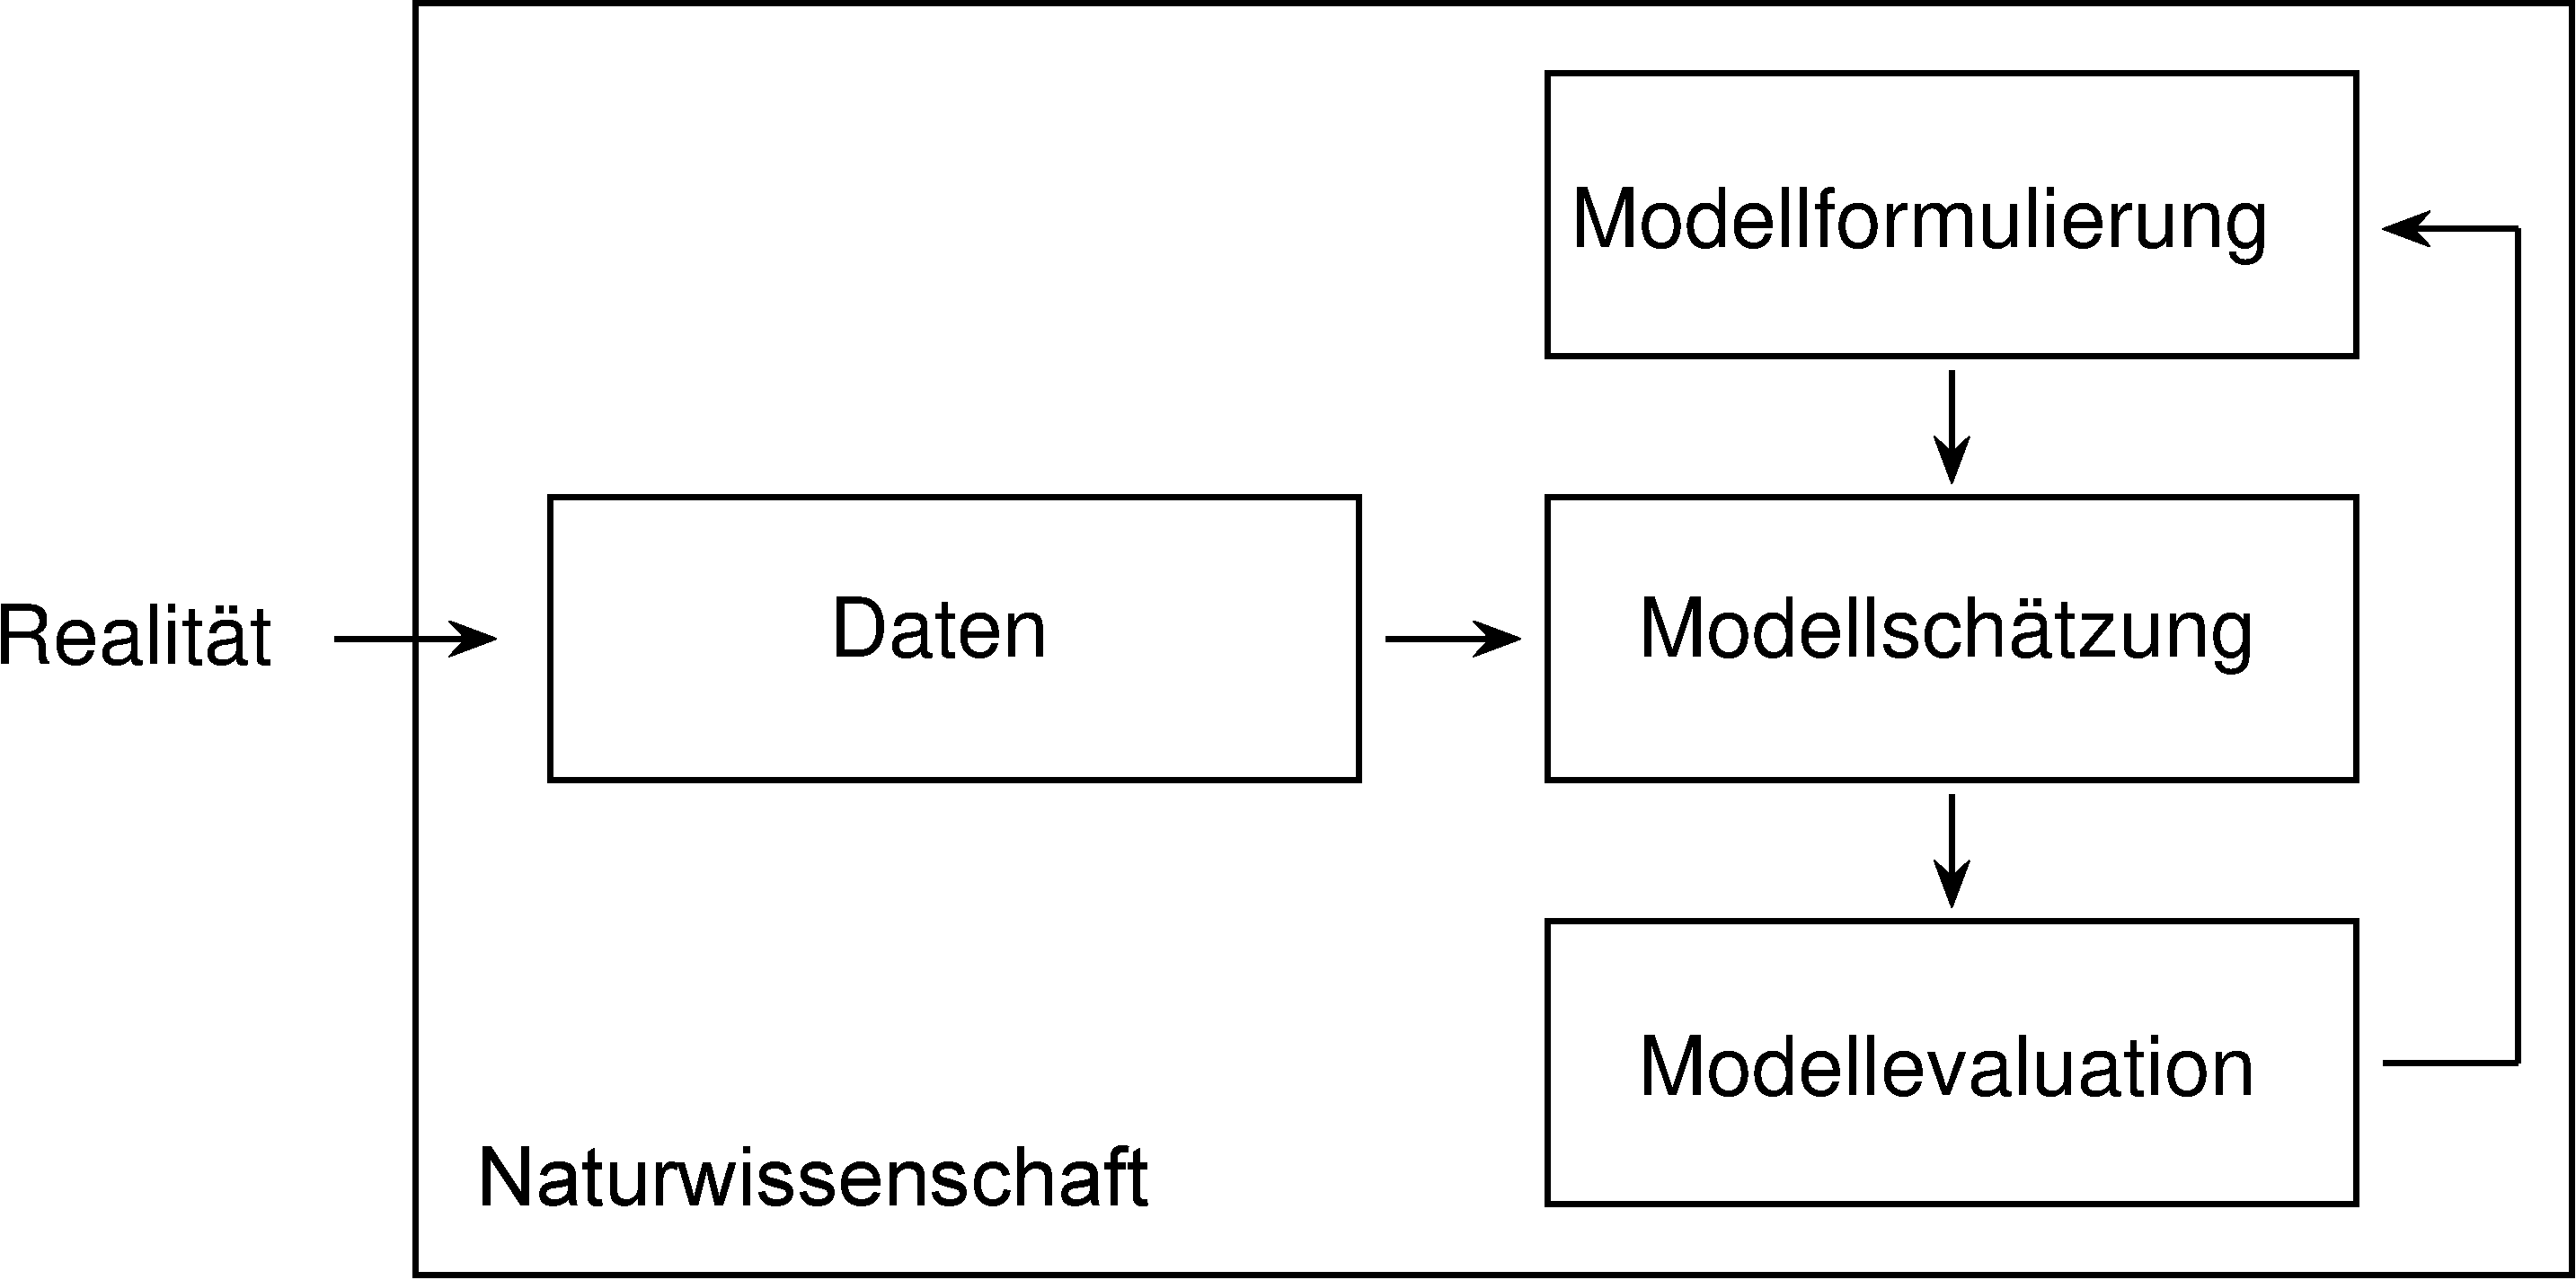
\includegraphics[width=0.9\linewidth]{4_Abbildungen/pfm_4_wissenschaft} \end{center}
\center
\vspace{2mm}
\large

\textcolor{darkblue}{Wo kommen die Zahlen her?}
\end{frame}

\begin{frame}{Überblick}
\protect\hypertarget{uxfcberblick-1}{}
\textcolor{darkblue}{Definitionsversuche}

\small
\justifying

``Measurement of magnitudes is, in its most general sense, any method by
which a unique and reciprocal correspondence is established bdtween all
or some of the magnitudes of a kind and all or some of the numbers,
integral, rational, or real as they may be''. \vspace{-1mm}

\flushright

Russell (1938)

\justifying

Measurement is ``the assigment of numerals to represent properties of
material systems other than number, in virtue of the laws governing
these properties''. \vspace{-1mm}

\flushright

Campbell and Jeffreys (1938)

\justifying

``Measurement is the assignment of numerals to objects or events
according to rules'' \vspace{-1mm}

\flushright

Stevens (1951)

\justifying

``Measurement of a property (\ldots) involves the assignment of numbers
to systems to represent that property''. \vspace{-1mm}

\flushright

Torgerson (1958)

\justifying

``Measurement has something to do with assigning numbers that correspond
to or represent or preserve certain observed relations.'' \vspace{-1mm}

\flushright

Roberts (1984)
\end{frame}

\begin{frame}{Überblick}
\protect\hypertarget{uxfcberblick-2}{}
\textcolor{darkblue}{Beispiel (1)}

\small

Temperaturmessung

\begin{itemize}
\item
  \justifying Messen der Temperatur eines Gegenstandes bedeutet, dem
  Gegenstand eine Zahl so zuordnen, dass die empirische Relation ``ist
  wärmer als'' in der Welt im Zahlenraum erhalten bleibt.
\item
  Sei \(M\) die Menge von Objekten und es gelte ``\(m\) ist wärmer als
  \(n\)'' für \(m,n\in M\), dann und nur dann wenn \(m\) als wärmer als
  \(n\) beurteilt wird. Dann möchte man bei der Messung der Temperatur
  von Objekten \(m\) und \(n\) so mithilfe einer Funktion \(f\) Zahlen
  zuordnen, dass gilt \begin{equation}
  m \mbox{ ist wärmer als } n \Leftrightarrow f(m) > f(n).
  \end{equation}
\item
  Eine solche Funktion heißt \emph{Thermometer}.
\end{itemize}
\end{frame}

\begin{frame}{Überblick}
\protect\hypertarget{uxfcberblick-3}{}
\textcolor{darkblue}{Beispiel (2)}

\small

Präferenzmessung

\begin{itemize}
\item
  \justifying Messen der Entscheidungsoptionspräferenzen eines Menschen
  (Lebewesens, Agenten), bedeutet diesem Zahlen so zuzuordnen, dass die
  empirische Relation ``wird präferiert über'' in der Welt im Zahlenraum
  erhalten bleibt.
\item
  Sei \(M\) die Menge von Entscheidungsoptionen und es gelte ``\(m\)
  wird präferiert \(n\)'' für \(m,n\in M\), dann und nur dann wenn \(m\)
  durch einen Menschen (ein Lebewesen, einen Agenten) über \(n\)
  präferiert wird. Dann möchte man bei der Messung von
  Entscheidungsoptionspräferenzen \(m\) und \(n\) so mithilfe einer
  Funktion \(f\) Zahlen zuordnen, dass gilt \begin{equation}
  m \mbox{ wird präferiert über  } n \Leftrightarrow f(m) > f(n).
  \end{equation}
\item
  Eine solche Funktion heißt \emph{Utility Function (Nutzenfunktion)}.
\end{itemize}
\end{frame}

\begin{frame}{Überblick}
\protect\hypertarget{uxfcberblick-4}{}
\textcolor{darkblue}{Beispiel (3)}

\small

Gewichtsmessung

\begin{itemize}
\item
  \justifying Messen des Gewichts eines Gegenstandes bedeutet, dem
  Gegenstand eine Zahl so zuordnen, dass die empirische Relation ``ist
  schwerer als'' in der Welt im Zahlenraum erhalten bleibt.
\item
  Sei \(M\) die Menge von Objekten und es gelte ``\(m\) ist schwerer als
  \(n\)'' für \(m,n\in M\), dann und nur dann wenn \(m\) als schwerer
  als \(n\) beurteilt wird. Dann möchte man bei der Messung des Gewichts
  von Objekten \(m\) und \(n\) so mithilfe einer Funktion \(f\) Zahlen
  zuordnen, dass gilt \begin{equation}
  m \mbox{ ist wärmer als } n \Leftrightarrow f(m) > f(n).
  \end{equation}
\item
  Eine solche Funktion heißt \emph{Waage}.
\item
  Weiterhin möchte man bei der Gewichtsmessung (Wiegen) auch sicher
  stellen, dass der Messprozess additiv ist, in dem Sinne, dass wenn man
  zwei Objekte kombiniert, ihr gemeinsames Gewicht der Summe ihrer
  einzelnen Gewichte entspricht. Formal sei \(\circ\) die Kombination
  zweier Objekte (z.B. das Nebeneinanderplatzieren in einer Waagschale).
  Dann soll die Waage nach Möglichkeit auch folgende Eigenschaft
  \begin{equation}
  f(m \mbox{ wird kombiniert mit } n) = f(m \circ n) \Leftrightarrow f(m) + f(b).
  \end{equation}
\end{itemize}

\flushright

\(\Rightarrow\) Additivität bei empirischen
Entscheidungsoptionspräferenzen kann, aber muss nicht, vorliegen.
\end{frame}

\begin{frame}{Überblick}
\protect\hypertarget{uxfcberblick-5}{}
\setstretch{1.8}

\textcolor{darkblue}{Repräsentationstheorie des Messens}

\begin{itemize}
\tightlist
\item
  Die Standardtheorie zu Messvorgängen und Inhalt dieser Einführung.
\end{itemize}

\textcolor{darkblue}{Qualitatives Relationssystem}

\begin{itemize}
\tightlist
\item
  Eine Menge von Eigenschaften von Objekten in der Realität und ihre
  Beziehungen.
\end{itemize}

\textcolor{darkblue}{Numerisches Relationssystem}

\begin{itemize}
\tightlist
\item
  Eine Mengen von Zahlen und ihre Beziehungen.
\end{itemize}

\textcolor{darkblue}{Homomorphismus}

\begin{itemize}
\tightlist
\item
  Eine Abbildung, die Beziehungen von Objekteigenschaften im Zahlenraum
  erhält.
\end{itemize}
\end{frame}

\begin{frame}{Überblick}
\protect\hypertarget{uxfcberblick-6}{}
\vfill

\begin{center}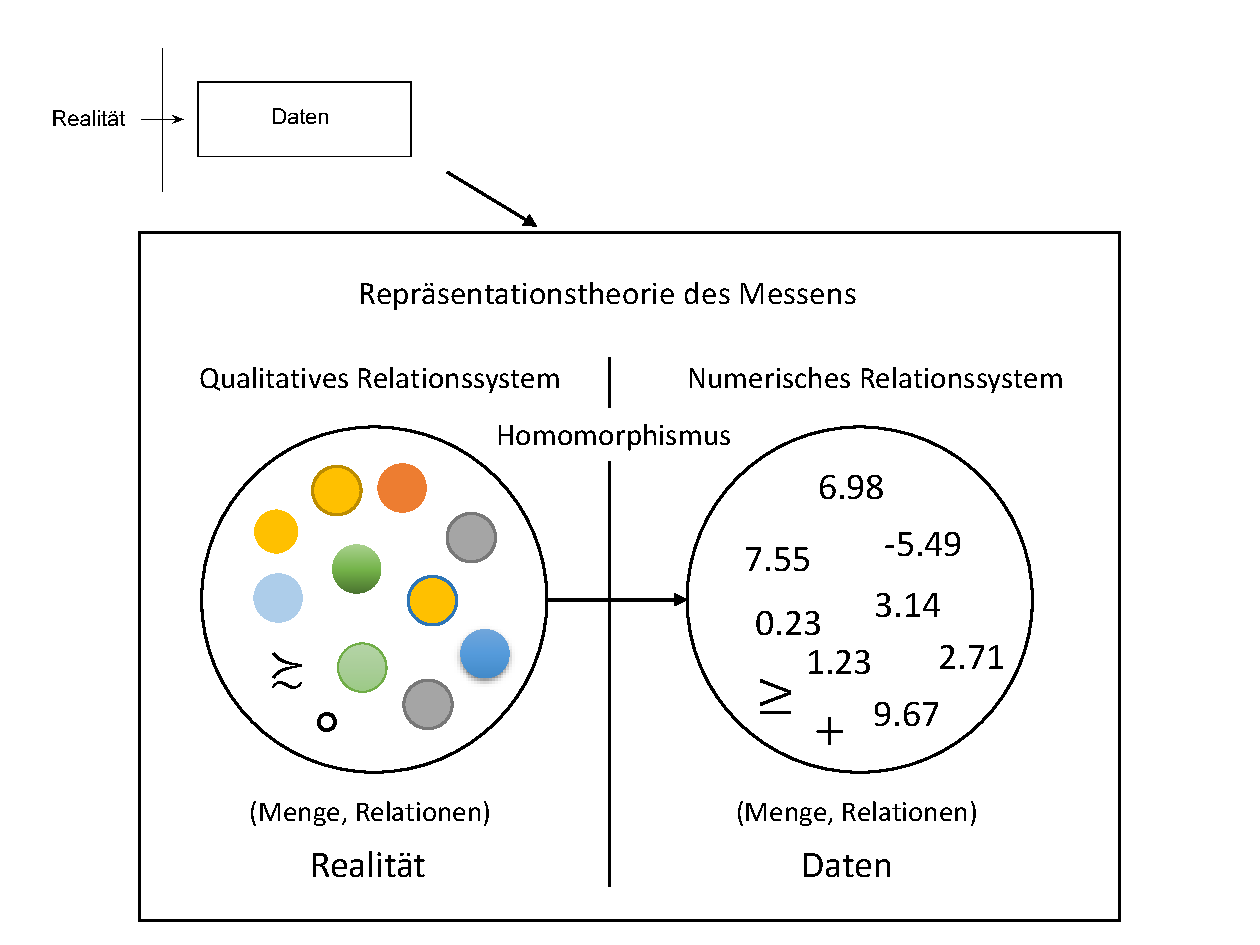
\includegraphics[width=0.9\linewidth]{4_Abbildungen/pfm_4_messtheorie} \end{center}
\end{frame}

\begin{frame}{Überblick}
\protect\hypertarget{uxfcberblick-7}{}
Bemerkungen

\small

\begin{itemize}
\item
  \justifying Messtheorie stellt einen logischen Apparat bereit, um
  qualitative Relationssysteme sinnvoll in numerische Relationssysteme
  abbilden zu können, also ein gegebenes qualitatives Relationssystem
  strutkurerhaltend im Bereich der Zahlen zu repräsentieren.
\item
  Messtheorie gibt allerdings insbesondere aber keine Antwort darauf,
  woher das qualitative Relationssystem kommt und wie es beschaffen ist,
  welche Art von Relationen für die betrachteten Eigenschaften von
  Objekten also gelten und welche nicht.
\item
  Messtheorie in ihrer klassischen Form betrachtet keine praktisch
  auftretenden Messfehler, dass also die gleiche Eigenschaftsausprägung
  eines Objektes manchmal auf eine Zahl und manchmal auf eine ähnliche,
  aber andere Zahl abgebildet wird; der Messvorgang selbst wird als
  (deterministische) Abbildung modelliert.
\item
  Sowohl Zufallsvariablen der Wahrscheinlichkeitstheorie als auch
  Homomorphismen der Messtheorie können als Modelle von Messvorgängen
  verstanden werden.
\end{itemize}
\end{frame}

\begin{frame}{Überblick}
\protect\hypertarget{uxfcberblick-8}{}
\vspace{1mm}

\textcolor{darkblue}{Skala}

Eine Skala ist die Einheit eines qualitativen Relationssystems, eines
numerischen Relationssystems und eines Homomorphismus. Die spezielle
Form von qualitativen Relationssystem, numerischen Relationssystem und
Homomorphismus bestimmt dabei die \emph{Skalenart}.

\vspace{3mm}

\textcolor{darkblue}{Skalenarten}

\setstretch{1.6}
\small
\begin{tabular}{ll}
Nominalskala    & Äquivalenzrelationen                                                \\
Ordinalskala    & Ordnungsrelationen                                                  \\
Intervallskala  & Ordnungsrelationen mit gleichen Abständen zwischen Skalenpunkten    \\
Verhältnisskala & Ordnungsrelationen mit gleichen Abständen und empirischem Nullpunkt \\
\end{tabular}

\flushright
\footnotesize

nach Stevens (1946)
\end{frame}

\begin{frame}{Überblick}
\protect\hypertarget{uxfcberblick-9}{}
\textcolor{darkblue}{Nominalskala}

Definition

\small

Der Homomorphismus einer Nominalskala ordnet Objekteigenschaften eines
qualitativen Relationssystems Zahlen zu, die so geartet sind, dass
gleiche Objekteigenschaften gleiche Zahlen und verschiedene
Objekteigenschaften verschiedene Zahlen erhalten.

\footnotesize
\flushright

nach Bortz and Schuster (2010)

\justifying
\normalsize

Eigenschaften

\small

\begin{itemize}
\tightlist
\item
  Die Zahlen einer Nominalskala sind Namen für Äquivalenzklassen ohne
  quantitative Bedeutung.
\item
  Je zwei Objekte des qualitativen und numerischen Relationssytems sind
  äquivalent oder nicht.
\end{itemize}

\normalsize

Beispiel

\small

Studienfach

\begin{itemize}
\tightlist
\item
  A studiert Psychologie, B studiert Psychologie, C studiert PNK.
\item
  A und B sind äquivalent, A und C sind nicht äquivalent, B und C sind
  nicht äquivalent
\item
  Nominalskala \(\{0,1\}\) mit 0 = Psychologie, 1 = PNK
\item
  A \(\mapsto 0\), B \(\mapsto 0\), C \(\mapsto 1\).
\end{itemize}
\end{frame}

\begin{frame}{Überblick}
\protect\hypertarget{uxfcberblick-10}{}
\textcolor{darkblue}{Ordinalskala}

Definition

\small

Der Homomorphismus einer Ordinalskala ordnet den Objekteigenschaften
eines qualitativen Relationssystems Zahlen zu, die so geartet sind, dass
von jeweils zwei Objekteigenschaft die stärker ausgeprägte Eigenschaft
die größere Zahl erhält.

\footnotesize
\flushright

nach Bortz and Schuster (2010)

\justifying
\normalsize

Eigenschaften

\small

\begin{itemize}
\tightlist
\item
  Die Zahlen einer Ordinalskals bilden eine Rangordnung im qualitativen
  Relationssystem ab.
\item
  Die Abstände zwischen zwei Rängen müssen nicht numerisch gleich sein.
\end{itemize}

\normalsize

Beispiel

\small

ESC 1974 Plätze

\begin{itemize}
\tightlist
\item
  \footnotesize 1. Platz: ABBA, 2. Platz: Cinquetti, 3. Platz: MacNeal.
\item
  Ordnungsrelation im qualitativen Relationssytem: ABBA \textgreater{}
  Cinquetti \textgreater{} MacNeal.
\item
  Ordinalskala \(\{1,2,3\}\) mit 1 = 1. Platz, 2 = 2. Platz, 3 = 3.
  Platz.
\item
  ABBA \(\mapsto 1\), Cinquetti \(\mapsto 2\), MacNeal \(\mapsto 3\).
\item
  ABER: ABBA = 24 Punkte, Cinquetti = 18 Punkte, MacNeal = 15 Punkte.
\end{itemize}
\end{frame}

\begin{frame}{Überblick}
\protect\hypertarget{uxfcberblick-11}{}
\textcolor{darkblue}{Intervallskala}

Definition

\small

Der Homomorphismus einer Intervallskala ordnet Objekteigenschaften eines
qualitativen Relationssystems Zahlen zu, die so geartet sind, dass die
Verhältnisse der Differenzen zwischen je zwei Objekteigenschaften den
Verhältnissen der Differenzen zwischen je zwei Zahlen des numerischen
Relationssystems entspricht.

\footnotesize
\flushright

nach Bortz and Schuster (2010)

\justifying
\normalsize

Beispiele und Eigenschaften \footnotesize

\begin{itemize}
\tightlist
\item
  Die Celsius Temperatuskala und die Fahrenheit Temperaturskala sind
  Intervallskalen
\item
  Es gilt \(T_F = 1.8\cdot T_C + 32\), also z.B. 10°C = 50°F, 20°C =
  68°F, 30°C = 86°F.
\item
  Bei Intervallskalen sind die Verhältnisse von Wertdifferenzen
  invariant, z.B. \begin{equation}
  \frac{30^{\circ}\mbox{C} - 10^{\circ}\mbox{C}}{30^{\circ}\mbox{C} - 20^{\circ}\mbox{C}} = \frac{20^{\circ}\mbox{C}}{10^{\circ}\mbox{C}} = 2 \mbox{ und }
  \frac{86^{\circ}\mbox{F} - 50^{\circ}\mbox{F}}{86^{\circ}\mbox{F} - 68^{\circ}\mbox{F}} = \frac{36^{\circ}\mbox{F}}{18^{\circ}\mbox{F}} = 2.
  \end{equation}
\item
  Bei Intervallskalen sind die Verhältnisse von Werten allerdings
  variant, z.B. \begin{equation}
  \frac{20^{\circ}\mbox{C}}{10^{\circ}\mbox{C}} = 2.00 \mbox{ und }
  \frac{68^{\circ}\mbox{F}}{50^{\circ}\mbox{F}} = 1.36.
  \end{equation}
\end{itemize}
\end{frame}

\begin{frame}{Skalenniveaus}
\protect\hypertarget{skalenniveaus}{}
\textcolor{darkblue}{Verhältnisskala}

Definition

\small

Die Verhältnisskala ordnet den Objekten des qualitativen Relationssytems
Zahlen zu, die so geartet sind, dass die Verhältnisse zwischen je zwei
Merkmalsausprägungen den Verhältnissen zwischen je zwei Zahlen der Skala
entspricht. Eine Verhältnisskala benötigt einen natürlichen Nullpunkt im
qualitativen und numerischen Relationssytem. \footnotesize \flushright
Bortz and Schuster (2010)

\justifying
\normalsize

Beispiele

\begin{itemize}
\tightlist
\item
  \small Die Kelvin Temperaturskala bildet physikalische Energiezustände
  auf Zahlen ab.
\item
  Die Längenskala in Meter bildet die physikalische Länge auf Zahlen ab.
\item
  Die Kilogrammskala bildet physikalische Zustände auf Zahlen ab.
\end{itemize}
\end{frame}

\begin{frame}{Überblick}
\protect\hypertarget{uxfcberblick-12}{}
Literaturempfehlung für ein vertieftes Verständnis \vfill

\begin{center}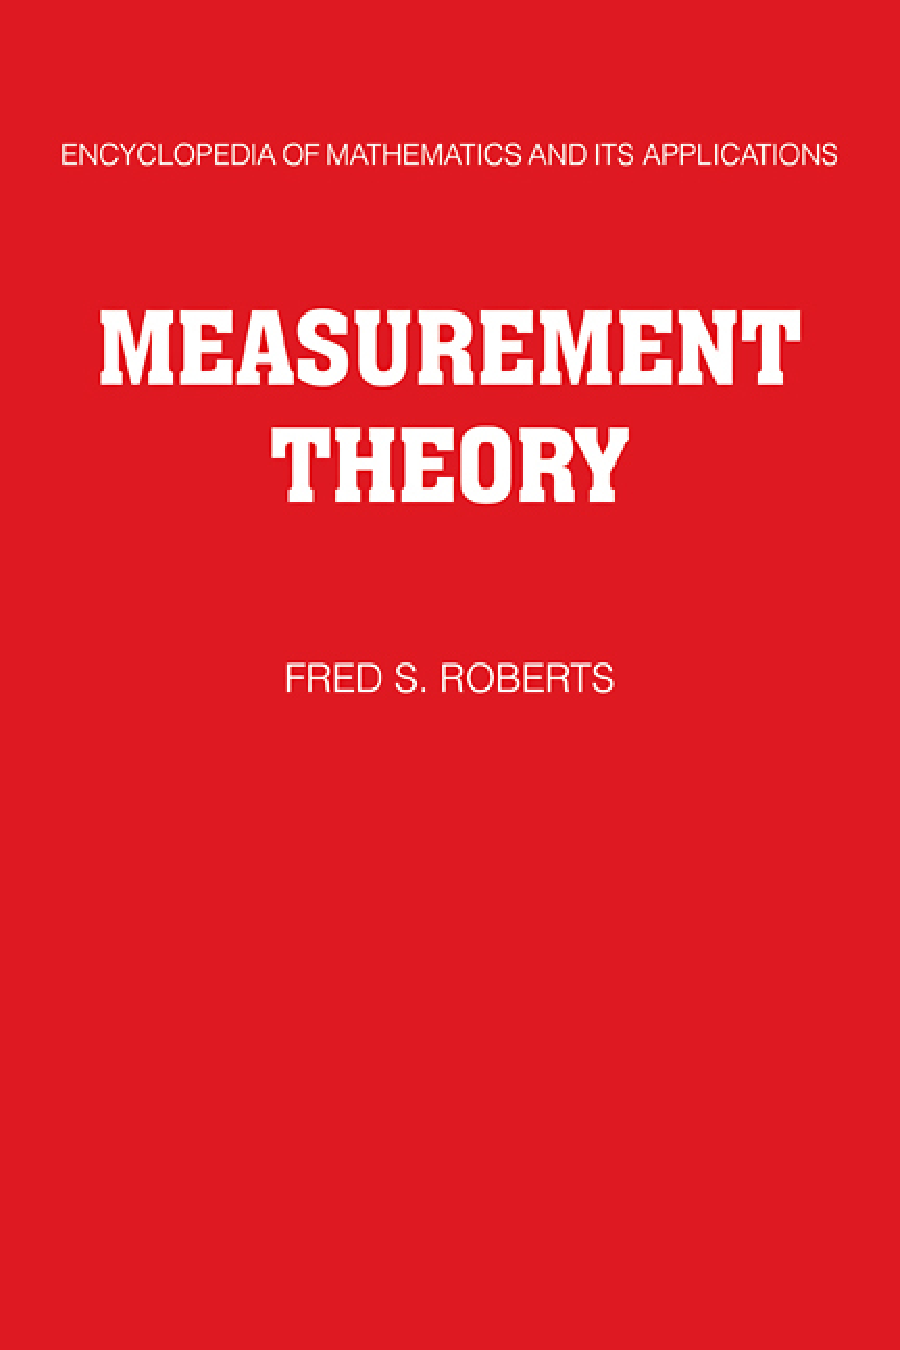
\includegraphics[width=0.35\linewidth]{4_Abbildungen/pfm_4_roberts} \end{center}
\footnotesize
\flushright

Roberts (1984)
\end{frame}

\begin{frame}{Überblick}
\protect\hypertarget{uxfcberblick-13}{}
\setstretch{2}

Vorlesungseinheiten zur Messtheorie

\begin{enumerate}
[(1)]
\setcounter{enumi}{3}
\tightlist
\item
  Einführung Messtheorie
\item
  Relationen
\item
  Grundprobleme
\item
  Skalenarten
\item
  Ordinalmessung
\item
  Extensivmessung
\item
  Bedeutsamkeit
\end{enumerate}
\end{frame}

\begin{frame}{}
\protect\hypertarget{section-4}{}
\Large
\setstretch{3}
\vfill

Überblick

\textbf{Selbstkontrollfragen} \vfill
\end{frame}

\begin{frame}{Selbstkontrollfragen}
\protect\hypertarget{selbstkontrollfragen}{}
\setstretch{2.5}
\footnotesize

\begin{enumerate}
\tightlist
\item
  Erläutern Sie den Begriff des Messens.
\item
  Nennen Sie drei Beispiele für Messungen.
\item
  Erläutern Sie den Begriff der Repräsentationstheorie des Messens.
\item
  Erläutern Sie den Begriff des qualitativen Relationssystems.
\item
  Erläutern Sie den Begriff des numerischen Relationssystems.
\item
  Erläutern Sie den Begriff des Homomorphismus.
\item
  Erläutern Sie den Begiff der Skalenart.
\item
  Erläutern Sie den Begriff der Nominalskala.
\item
  Erläutern Sie den Begriff der Ordinalskala.
\item
  Erläutern Sie den Begriff der Intervallskala.
\item
  Erläutern Sie den Begriff der Verhältnisskala.
\end{enumerate}
\end{frame}

\begin{frame}{Referenzen}
\protect\hypertarget{referenzen}{}
\footnotesize

\hypertarget{refs}{}
\begin{CSLReferences}{1}{0}
\leavevmode\vadjust pre{\hypertarget{ref-bortz_2010}{}}%
Bortz, Jürgen, and Christof Schuster. 2010. \emph{Statistik Für {Human}-
Und {Sozialwissenschaftler}}. 7., vollständig überarbeitete und
erweiterte Auflage. Springer-{Lehrbuch}. Berlin Heidelberg: Springer.

\leavevmode\vadjust pre{\hypertarget{ref-campbell_1938}{}}%
Campbell, N. R., and H. Jeffreys. 1938. {``Symposium: {Measurement} and
Its {Importance} for {Philosophy}.''} \emph{Aristotelian Society
Supplementary Volume} 17 (1): 121--50.
\url{https://doi.org/10.1093/aristoteliansupp/17.1.121}.

\leavevmode\vadjust pre{\hypertarget{ref-roberts_1984}{}}%
Roberts, Fred S. 1984. \emph{Measurement Theory with Applications to
Decisionmaking, Utility, and the Social Sciences}. Encyclopedia of
Mathematics and Its Applications ; {Section}, {Mathematics} and the
Social Sciences, v. 7. Cambridge {[}Cambridgeshire{]} ; New York, NY,
USA: Cambridge University Press.

\leavevmode\vadjust pre{\hypertarget{ref-russell_1938}{}}%
Russell, Bertrand. 1938. \emph{Principles of {Mathematics}}. Routledge
Classics. London: Routledge.

\leavevmode\vadjust pre{\hypertarget{ref-stevens_1946}{}}%
Stevens, S. S. 1946. {``On the {Theory} of {Scales} of {Measurement}.''}
\emph{Science, New Series} 103 (2684): 677--80.
\url{http://www.jstor.org/stable/1671815}.

\leavevmode\vadjust pre{\hypertarget{ref-stevens_1951}{}}%
---------. 1951. {``Mathematics, Measurement, and Psychophysics.''} In
\emph{Handbook of {Experimental} {Psychology}}, 1--49.

\leavevmode\vadjust pre{\hypertarget{ref-torgerson_1958}{}}%
Torgerson, W. S. 1958. \emph{Theory and {Methods} of {Scaling}}. New
York: Wiley.

\end{CSLReferences}
\end{frame}

\end{document}
